% ==============================================================================
% Topic 04: Microcontrollers
% GRADE: A | PRIORITY: [SHOW OFF] (YOUR STRONGEST SUBJECT!)
% ==============================================================================

\section{Microcontrollers | 微控制器}

\begin{tipbox}[\textcolor{green}{\textbf{[STAR]}} GRADE A DETECTED: SHOW OFF MODE / 成绩A:展示模式]
\textbf{[CN]} 微控制器是你的\textbf{最强科目} (A)!这是你的主场,\textbf{主动把话题引向ESP32}!\\
\textbf{[EN]} MIK is your \textbf{STRONGEST subject} (A)! This is YOUR domain. \textbf{Pivot to ESP32 immediately}!\\
\textbf{Power Move}: 任何中断/ADC/通信问题 → ``In my thesis, I implemented this on ESP32...``
\end{tipbox}

\begin{defbox}{Chapter Overview | 章节概览}
微控制器是嵌入式系统的核心,本章作为最强科目,将深入覆盖所有考点:
\begin{enumerate}
    \item Timer/Counter --- PWM生成与频率测量
    \item GPIO --- 通用输入输出配置
    \item ADC --- 模数转换与传感器接口
    \item PWM --- 脉宽调制与电机控制
    \item Interrupts --- 中断处理机制
    \item UART --- 串口通信协议
    \item 综合应用 --- ESP32 IoT传感器系统
\end{enumerate}
\tcblower
Microcontrollers are the heart of embedded systems. This chapter covers all exam topics comprehensively as your strongest subject.
\end{defbox}

% ==============================================================================
\subsection{Timer/Counter | 定时器/计数器}
% ==============================================================================

\begin{formulabox}{Timer Fundamentals | 定时器基础公式}
\textbf{定时器溢出时间 (Timer Overflow Period):}
\begin{equation}
    T_{overflow} = \frac{2^n \times \text{Prescaler}}{f_{clk}}
\end{equation}

\textbf{PWM频率计算 (PWM Frequency):}
\begin{equation}
    f_{PWM} = \frac{f_{clk}}{\text{Prescaler} \times (TOP + 1)}
\end{equation}

\textbf{输入捕获频率测量 (Input Capture):}
\begin{equation}
    f_{signal} = \frac{f_{clk}}{\text{Prescaler} \times \Delta_{capture}}
\end{equation}

\begin{itemize}
    \item $n$ --- 定时器位数 (8-bit: 256, 16-bit: 65536)
    \item $f_{clk}$ --- 系统时钟频率
    \item TOP --- 定时器最大计数值(可配置)
    \item Prescaler --- 预分频值 (1, 8, 64, 256, 1024...)
\end{itemize}
\tcblower
Timer period depends on bit-width, prescaler, and clock frequency.
\end{formulabox}

\begin{studybox}{Blackboard Challenge 1: PWM Frequency | PWM频率计算}
\textbf{Problem:} ESP32时钟80MHz,使用LEDC模块,13-bit分辨率,要产生50Hz的舵机控制信号。求分频值。

\textbf{Step-by-step Solution:}
\begin{enumerate}
    \item 已知参数: $f_{clk} = 80MHz$, $f_{PWM} = 50Hz$, 分辨率 = 13-bit
    \item 13-bit分辨率意味着: $TOP = 2^{13} - 1 = 8191$
    \item 应用公式: $f_{PWM} = \frac{f_{clk}}{\text{Prescaler} \times (TOP + 1)}$
    \item 变换求Prescaler: 
    \begin{align}
        \text{Prescaler} &= \frac{f_{clk}}{f_{PWM} \times (TOP + 1)} \\
        &= \frac{80 \times 10^6}{50 \times 8192} \\
        &= \frac{80000000}{409600} \\
        &= 195.3125
    \end{align}
    \item 实际选择: Prescaler = 195 或 196(取整)
    \item 验证: $f_{PWM} = \frac{80MHz}{195 \times 8192} = 50.08Hz$ \checkmark
\end{enumerate}
\tcblower
\textbf{Answer:} $\boxed{\text{Prescaler} \approx 195}$

\textbf{ESP32 LEDC配置代码要点:}
\begin{verbatim}
ledc_timer_config_t timer = {
    .duty_resolution = LEDC_TIMER_13_BIT,
    .freq_hz = 50,  // 自动计算分频
    .speed_mode = LEDC_HIGH_SPEED_MODE
};
\end{verbatim}
\end{studybox}

\begin{studybox}{Blackboard Challenge 2: Timer Overflow | 定时器溢出}
\textbf{Problem:} AVR ATmega328P (Arduino Uno), $f_{clk} = 16MHz$, Timer1 (16-bit), Prescaler = 1024。求溢出周期和最大可测时间。

\textbf{Step-by-step Solution:}
\begin{enumerate}
    \item 16-bit定时器最大计数: $2^{16} = 65536$
    \item 每个计数的时间: $T_{tick} = \frac{\text{Prescaler}}{f_{clk}} = \frac{1024}{16MHz} = 64\mu s$
    \item 溢出周期: $T_{overflow} = 65536 \times 64\mu s = 4.194s$
    \item 定时器频率: $f_{timer} = \frac{1}{64\mu s} = 15.625kHz$
\end{enumerate}
\tcblower
\textbf{Answer:} $\boxed{T_{overflow} = 4.194s}$ (约4.2秒溢出一次)

\textbf{应用:} 可测量最长约4秒的脉冲宽度或周期
\end{studybox}

\begin{warnbox}{Mnemonic: Timer Prescaler | 记忆口诀}
\textbf{口诀: ``预分频大,周期长;位数高,范围广''}

\begin{itemize}
    \item 预分频器(Prescaler): 像变速箱,档位越高(值越大),转得越慢
    \item 定时器位数: 像油箱容量,越大能跑越久
    \item 时钟频率: 像发动机转速,越快计数越快
\end{itemize}

\textbf{快速估算技巧:}
\begin{itemize}
    \item 8-bit + 1024分频 @ 16MHz $\approx$ 16ms溢出
    \item 16-bit + 1024分频 @ 16MHz $\approx$ 4s溢出
\end{itemize}
\tcblower
Higher prescaler = longer period; More bits = wider range
\end{warnbox}

% ==============================================================================
\subsection{GPIO Configuration | GPIO配置}
% ==============================================================================

\begin{formulabox}{GPIO Modes | GPIO模式}
\textbf{基本配置模式:}
\begin{center}
\renewcommand{\arraystretch}{1.3}
\begin{tabular}{|l|l|l|}
\hline
\textbf{Mode} & \textbf{中文} & \textbf{应用场景} \\
\hline
Input & 输入模式 & 读取按键、传感器数字信号 \\
\hline
Output & 输出模式 & 驱动LED、继电器 \\
\hline
Input Pull-up & 上拉输入 & 按键(低电平有效) \\
\hline
Input Pull-down & 下拉输入 & 按键(高电平有效) \\
\hline
Open-drain & 开漏输出 & I2C总线、电平转换 \\
\hline
Analog & 模拟模式 & ADC输入、DAC输出 \\
\hline
Alternate Function & 复用功能 & UART/SPI/I2C/PWM \\
\hline
\end{tabular}
\end{center}
\tcblower
GPIO can be configured as input, output, or alternate functions with optional pull resistors.
\end{formulabox}

\begin{studybox}{Blackboard Challenge 3: Pull-up Resistor | 上拉电阻计算}
\textbf{Problem:} 按键接GPIO,使用内部上拉。ESP32内部上拉约45k$\Omega$,按键按下时GPIO接地。求按下和释放时的电压,以及功耗。

\textbf{Step-by-step Solution:}
\begin{enumerate}
    \item \textbf{按键释放时 (Open):}
    \begin{itemize}
        \item 无电流流过,GPIO通过上拉接3.3V
        \item $V_{GPIO} = 3.3V$ (逻辑高)
        \item 功耗: $P = 0W$
    \end{itemize}
    
    \item \textbf{按键按下时 (Closed):}
    \begin{itemize}
        \item GPIO直接接地
        \item $V_{GPIO} = 0V$ (逻辑低)
        \item 电流: $I = \frac{3.3V}{45k\Omega} = 73.3\mu A$
        \item 功耗: $P = 3.3V \times 73.3\mu A = 242\mu W$
    \end{itemize}
\end{enumerate}
\tcblower
\textbf{Answer:} 
$\boxed{V_{released} = 3.3V, \quad V_{pressed} = 0V, \quad P_{pressed} = 242\mu W}$

\textbf{设计考虑:} 低功耗应用应使用外部上拉(100k$\Omega$+)减少电流
\end{studybox}

\begin{defbox}{GPIO Register Architecture | GPIO寄存器架构}
\textbf{典型GPIO寄存器组 (以STM32为例):}
\begin{itemize}
    \item \texttt{GPIOx\_MODER} --- 模式寄存器 (Input/Output/AF/Analog)
    \item \texttt{GPIOx\_OTYPER} --- 输出类型 (Push-pull/Open-drain)
    \item \texttt{GPIOx\_OSPEEDR} --- 输出速度 (Low/Medium/High/Very High)
    \item \texttt{GPIOx\_PUPDR} --- 上拉/下拉配置
    \item \texttt{GPIOx\_IDR} --- 输入数据寄存器 (只读)
    \item \texttt{GPIOx\_ODR} --- 输出数据寄存器
    \item \texttt{GPIOx\_BSRR} --- 位设置/复位寄存器 (原子操作)
\end{itemize}

\textbf{ESP32 GPIO Matrix特点:}
\begin{itemize}
    \item 任意GPIO可映射到任意外设功能(通过GPIO Matrix)
    \item 支持RTC域GPIO (Deep Sleep时仍可工作)
    \item 部分GPIO仅支持输入 (GPIO34-39)
\end{itemize}
\tcblower
GPIO registers control mode, speed, pull resistors, and data. ESP32 has flexible GPIO matrix for peripheral mapping.
\end{defbox}

\begin{warnbox}{Mnemonic: GPIO Modes | 记忆口诀}
\textbf{口诀: ``上拉高,下拉低;开漏要外拉,推挽可直驱''}

\begin{itemize}
    \item \textbf{上拉输入:} 默认高电平,按键按下变低(低电平有效)
    \item \textbf{下拉输入:} 默认低电平,按键按下变高(高电平有效)
    \item \textbf{开漏输出:} 只能拉低,拉高需外部上拉(用于I2C、电平转换)
    \item \textbf{推挽输出:} 可主动拉高拉低,驱动能力强
\end{itemize}

\textbf{ESP32 GPIO陷阱:}
\begin{itemize}
    \item GPIO6-11: 连接Flash,勿使用!
    \item GPIO34-39: 仅输入,无上拉
    \item GPIO0/2/15: Boot模式引脚,使用需小心
\end{itemize}
\tcblower
Pull-up = default HIGH; Pull-down = default LOW; Open-drain needs external pull-up.
\end{warnbox}

% ==============================================================================
\subsection{ADC | 模数转换器}
% ==============================================================================

\begin{formulabox}{ADC Fundamentals | ADC基础公式}
\textbf{分辨率与量化步长 (Resolution and LSB):}
\begin{equation}
    \text{LSB} = \frac{V_{ref}}{2^n} \quad \text{(最小可分辨电压)}
\end{equation}

\textbf{数字值与电压转换 (Digital to Voltage):}
\begin{equation}
    V_{analog} = \frac{\text{ADC\_Value} \times V_{ref}}{2^n}
\end{equation}

\textbf{电压转数字值 (Voltage to Digital):}
\begin{equation}
    \text{ADC\_Value} = \frac{V_{analog} \times 2^n}{V_{ref}}
\end{equation}

\textbf{采样率与奈奎斯特 (Sampling Rate):}
\begin{equation}
    f_s \geq 2 \times f_{max} \quad \text{(奈奎斯特定理)}
\end{equation}

\begin{itemize}
    \item $n$ --- ADC位数 (ESP32: 12-bit, STM32: 12-bit)
    \item $V_{ref}$ --- 参考电压 (ESP32: 1.1V内部或3.3V衰减后)
    \item LSB --- Least Significant Bit (最低有效位)
\end{itemize}
\tcblower
ADC resolution determines the smallest voltage step. Higher bits = finer resolution.
\end{formulabox}

\begin{studybox}{Blackboard Challenge 4: ADC Resolution | ADC分辨率计算}
\textbf{Problem:} ESP32 ADC 12-bit,参考电压3.3V(11dB衰减)。求:(a)分辨率,(b)1.65V对应的ADC值,(c)ADC值2048对应的电压。

\textbf{Step-by-step Solution:}
\begin{enumerate}
    \item \textbf{(a) 分辨率/LSB:}
    \begin{equation}
        \text{LSB} = \frac{3.3V}{2^{12}} = \frac{3.3V}{4096} = 0.806mV
    \end{equation}
    
    \item \textbf{(b) 1.65V对应的ADC值:}
    \begin{equation}
        \text{ADC} = \frac{1.65V \times 4096}{3.3V} = \frac{6758.4}{3.3} = 2048
    \end{equation}
    
    \item \textbf{(c) ADC值2048对应的电压:}
    \begin{equation}
        V = \frac{2048 \times 3.3V}{4096} = 1.65V
    \end{equation}
    
    \item \textbf{验证:} 2048是4096的一半,对应$V_{ref}$的一半 \checkmark
\end{enumerate}
\tcblower
\textbf{Answer:} 
$\boxed{\text{(a) LSB} = 0.806mV, \quad \text{(b) ADC} = 2048, \quad \text{(c) V} = 1.65V}$
\end{studybox}

\begin{studybox}{Blackboard Challenge 5: Temperature Sensor | 温度传感器ADC}
\textbf{Problem:} NTC热敏电阻与10k$\Omega$电阻分压,接ESP32 ADC。NTC在25C时10k$\Omega$,温度升高阻值降低。ADC读数3000时,求NTC阻值和估算温度。

\textbf{Step-by-step Solution:}
\begin{enumerate}
    \item \textbf{电路分析:} $V_{out} = 3.3V \times \frac{R_{fixed}}{R_{NTC} + R_{fixed}}$
    
    \item \textbf{从ADC值求电压:}
    \begin{equation}
        V_{out} = \frac{3000 \times 3.3V}{4096} = 2.417V
    \end{equation}
    
    \item \textbf{从电压求NTC阻值:}
    \begin{align}
        2.417 &= 3.3 \times \frac{10k}{R_{NTC} + 10k} \\
        R_{NTC} + 10k &= \frac{3.3 \times 10k}{2.417} = 13.65k \\
        R_{NTC} &= 3.65k\Omega
    \end{align}
    
    \item \textbf{温度估算 (Steinhart-Hart简化):}
    \begin{itemize}
        \item NTC阻值降低,说明温度升高
        \item 10k$\Omega$ @ 25C $\rightarrow$ 3.65k$\Omega$ 约对应50-60C
    \end{itemize}
\end{enumerate}
\tcblower
\textbf{Answer:} $\boxed{R_{NTC} = 3.65k\Omega}$ (温度约50-60C)
\end{studybox}

\begin{warnbox}{Mnemonic: ADC | 记忆口诀}
\textbf{口诀: ``位数定精度,参考定范围;采样要翻倍,混叠会捣乱''}

\begin{itemize}
    \item \textbf{位数定精度:} 12-bit = 4096级 = 0.024\%精度
    \item \textbf{参考定范围:} $V_{ref}$决定可测最大电压
    \item \textbf{采样要翻倍:} $f_s \geq 2f_{max}$ (奈奎斯特)
    \item \textbf{混叠会捣乱:} 采样率不够会产生假信号
\end{itemize}

\textbf{ESP32 ADC注意事项:}
\begin{itemize}
    \item ADC2在WiFi使用时不可用!
    \item 非线性需要校准(esp\_adc\_cal)
    \item 衰减设置: 0dB(1.1V), 2.5dB(1.5V), 6dB(2.2V), 11dB(3.3V)
\end{itemize}
\tcblower
Bits = precision; $V_{ref}$ = range; Sample rate must be $\geq 2\times$ max frequency.
\end{warnbox}

% ==============================================================================
\subsection{PWM | 脉宽调制}
% ==============================================================================

\begin{formulabox}{PWM Fundamentals | PWM基础公式}
\textbf{占空比 (Duty Cycle):}
\begin{equation}
    D = \frac{T_{on}}{T_{period}} \times 100\% = \frac{T_{on}}{T_{on} + T_{off}} \times 100\%
\end{equation}

\textbf{平均电压 (Average Voltage):}
\begin{equation}
    V_{avg} = D \times V_{max} = \frac{T_{on}}{T_{period}} \times V_{max}
\end{equation}

\textbf{PWM分辨率与占空比精度:}
\begin{equation}
    \text{Duty Step} = \frac{100\%}{2^n} \quad \text{(n-bit分辨率)}
\end{equation}

\textbf{舵机控制 (Servo):}
\begin{equation}
    \text{Pulse Width: } 1ms \text{ (0 deg)} \leftrightarrow 1.5ms \text{ (90 deg)} \leftrightarrow 2ms \text{ (180 deg)}
\end{equation}
\tcblower
PWM duty cycle controls average voltage. Higher resolution = finer control.
\end{formulabox}

\begin{studybox}{Blackboard Challenge 6: Servo Control | 舵机控制计算}
\textbf{Problem:} 使用ESP32 LEDC控制舵机,PWM频率50Hz,13-bit分辨率。求0 deg、90 deg、180 deg对应的占空比和寄存器值。

\textbf{Step-by-step Solution:}
\begin{enumerate}
    \item \textbf{PWM周期:} $T = \frac{1}{50Hz} = 20ms$
    
    \item \textbf{占空比计算:}
    \begin{itemize}
        \item 0 deg (1ms): $D = \frac{1ms}{20ms} = 5\%$
        \item 90 deg (1.5ms): $D = \frac{1.5ms}{20ms} = 7.5\%$
        \item 180 deg (2ms): $D = \frac{2ms}{20ms} = 10\%$
    \end{itemize}
    
    \item \textbf{寄存器值计算 (13-bit = 8192):}
    \begin{itemize}
        \item 0 deg: $\text{Value} = 0.05 \times 8192 = 409.6 \approx 410$
        \item 90 deg: $\text{Value} = 0.075 \times 8192 = 614.4 \approx 614$
        \item 180 deg: $\text{Value} = 0.10 \times 8192 = 819.2 \approx 819$
    \end{itemize}
\end{enumerate}
\tcblower
\textbf{Answer:} 
$\boxed{0^{\circ} \rightarrow 410, \quad 90^{\circ} \rightarrow 614, \quad 180^{\circ} \rightarrow 819}$

\textbf{角度到寄存器值的线性公式:}
$\text{Value} = 410 + \frac{\theta}{180} \times (819 - 410) = 410 + 2.27\theta$
\end{studybox}

\begin{studybox}{Blackboard Challenge 7: LED Dimming | LED调光}
\textbf{Problem:} ESP32控制LED,要求256级亮度调节(8-bit感知),但LEDC用13-bit。设计映射关系实现感知线性亮度。

\textbf{Step-by-step Solution:}
\begin{enumerate}
    \item \textbf{问题:} 人眼对亮度感知是对数关系,线性PWM会感觉不均匀
    
    \item \textbf{解决方案 --- Gamma校正:}
    \begin{equation}
        \text{PWM}_{output} = \left(\frac{\text{Level}}{255}\right)^\gamma \times 8191
    \end{equation}
    
    \item \textbf{常用$\gamma = 2.2$:}
    \begin{itemize}
        \item Level 0: $(\frac{0}{255})^{2.2} \times 8191 = 0$
        \item Level 128: $(\frac{128}{255})^{2.2} \times 8191 = 1853$
        \item Level 255: $(\frac{255}{255})^{2.2} \times 8191 = 8191$
    \end{itemize}
    
    \item \textbf{查表法实现:} 预计算256个值存入数组
\end{enumerate}
\tcblower
\textbf{Answer:} $\boxed{\text{PWM} = \left(\frac{\text{Level}}{255}\right)^{2.2} \times 8191}$

使用Gamma校正实现感知线性的亮度调节。
\end{studybox}

\begin{warnbox}{Mnemonic: PWM | 记忆口诀}
\textbf{口诀: ``高时间比总时间,平均电压占比算''}

\begin{itemize}
    \item 占空比 = 高电平时间 / 总周期
    \item 平均电压 = 占空比 $\times$ 峰值电压
    \item 频率越高,滤波后越平滑
\end{itemize}

\textbf{舵机口诀: ``一毫零度,二毫满转,中间1.5''}
\begin{itemize}
    \item 1ms脉宽 $\rightarrow$ 0 deg
    \item 1.5ms脉宽 $\rightarrow$ 90 deg
    \item 2ms脉宽 $\rightarrow$ 180 deg
\end{itemize}
\tcblower
Duty = ON time / Period; Servo: 1ms=0 deg, 1.5ms=90 deg, 2ms=180 deg
\end{warnbox}

% ==============================================================================
\subsection{Interrupts | 中断}
% ==============================================================================

\begin{formulabox}{Interrupt vs Polling | 中断与轮询对比}
\begin{center}
\renewcommand{\arraystretch}{1.3}
\begin{tabular}{|l|l|l|}
\hline
\textbf{特性} & \textbf{Polling (轮询)} & \textbf{Interrupt (中断)} \\
\hline
CPU占用 & 持续检查,占用高 & 事件触发,占用低 \\
\hline
响应时间 & 取决于轮询间隔 & 几乎立即($\mu$s级) \\
\hline
实时性 & 差 & 好 \\
\hline
功耗 & 高(CPU一直运行) & 低(可休眠等待) \\
\hline
编程复杂度 & 简单 & 需处理并发 \\
\hline
适用场景 & 简单任务、非实时 & 按键、通信、定时 \\
\hline
\end{tabular}
\end{center}
\tcblower
Polling: CPU continuously checks; Interrupt: Event-driven, efficient for real-time.
\end{formulabox}

\begin{defbox}{Interrupt Handling | 中断处理流程}
\textbf{中断响应过程:}
\begin{enumerate}
    \item \textbf{中断请求 (IRQ):} 外设产生中断信号
    \item \textbf{中断响应:} CPU完成当前指令,保存上下文(PC, SR, 寄存器)
    \item \textbf{中断向量:} 查表获取ISR入口地址
    \item \textbf{执行ISR:} 运行中断服务程序
    \item \textbf{中断返回:} 恢复上下文,继续主程序
\end{enumerate}

\textbf{中断延迟 (Interrupt Latency):}
\begin{equation}
    T_{latency} = T_{sync} + T_{save} + T_{vector} + T_{ISR\_entry}
\end{equation}

\textbf{ESP32中断优先级:} 1-7级(7最高),支持嵌套中断

\textbf{ISR编写原则:}
\begin{itemize}
    \item 尽量短小,只做标记
    \item 避免使用阻塞函数(delay, printf)
    \item 使用volatile声明共享变量
    \item ESP32: 使用IRAM\_ATTR放入IRAM
\end{itemize}
\tcblower
ISR should be short, non-blocking, and use volatile for shared variables.
\end{defbox}

\begin{studybox}{Blackboard Challenge 8: Interrupt Latency | 中断延迟分析}
\textbf{Problem:} ESP32 @ 240MHz,按键触发GPIO中断。假设上下文保存需要20个时钟周期,向量查找10周期,ISR入口10周期。求最小中断延迟。

\textbf{Step-by-step Solution:}
\begin{enumerate}
    \item \textbf{时钟周期时间:}
    \begin{equation}
        T_{cycle} = \frac{1}{240MHz} = 4.17ns
    \end{equation}
    
    \item \textbf{总周期数:} $20 + 10 + 10 = 40$ cycles
    
    \item \textbf{中断延迟:}
    \begin{equation}
        T_{latency} = 40 \times 4.17ns = 166.8ns
    \end{equation}
    
    \item \textbf{实际考虑:}
    \begin{itemize}
        \item 流水线清空: +20 cycles
        \item Cache Miss: +100 cycles (if ISR not in IRAM)
        \item 实际延迟: 约200-500ns
    \end{itemize}
\end{enumerate}
\tcblower
\textbf{Answer:} $\boxed{T_{latency,min} \approx 167ns}$ (理想情况)

实际约0.5-2$\mu$s,取决于Cache状态和ISR位置。
\end{studybox}

\begin{warnbox}{Mnemonic: Interrupt | 记忆口诀}
\textbf{口诀: ``轮询费CPU,中断省功耗;ISR要短快,volatile不能少''}

\textbf{中断处理五字诀: ``请响向执返''}
\begin{enumerate}
    \item 请 --- 中断请求
    \item 响 --- CPU响应
    \item 向 --- 查向量表
    \item 执 --- 执行ISR
    \item 返 --- 中断返回
\end{enumerate}

\textbf{ISR三不要:}
\begin{itemize}
    \item 不要delay
    \item 不要printf
    \item 不要太长
\end{itemize}
\tcblower
Polling wastes CPU; Interrupts save power; ISR must be short with volatile variables.
\end{warnbox}

% ==============================================================================
\subsection{UART | 串口通信}
% ==============================================================================

\begin{formulabox}{UART Fundamentals | UART基础}
\textbf{波特率计算 (Baud Rate):}
\begin{equation}
    \text{Baud Rate} = \frac{f_{clk}}{\text{Divisor} \times 16}
\end{equation}

\textbf{位时间 (Bit Time):}
\begin{equation}
    T_{bit} = \frac{1}{\text{Baud Rate}}
\end{equation}

\textbf{帧格式 (Frame Format):}
\begin{center}
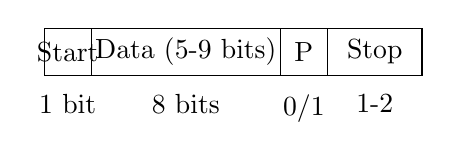
\begin{tikzpicture}[scale=0.6]
    \draw (0,0) rectangle (1,1); \node at (0.5,0.5) {Start};
    \draw (1,0) rectangle (5,1); \node at (3,0.5) {Data (5-9 bits)};
    \draw (5,0) rectangle (6,1); \node at (5.5,0.5) {P};
    \draw (6,0) rectangle (8,1); \node at (7,0.5) {Stop};
    \node[below] at (0.5,-0.2) {1 bit};
    \node[below] at (3,-0.2) {8 bits};
    \node[below] at (5.5,-0.2) {0/1};
    \node[below] at (7,-0.2) {1-2};
\end{tikzpicture}
\end{center}

\textbf{常见配置:} 8N1 = 8数据位 + 无校验 + 1停止位

\textbf{有效数据率:}
\begin{equation}
    \text{Effective Rate} = \frac{\text{Data bits}}{\text{Total bits}} \times \text{Baud Rate}
\end{equation}
\tcblower
UART frame: Start bit + Data + Parity (optional) + Stop bit(s)
\end{formulabox}

\begin{studybox}{Blackboard Challenge 9: UART Baud Rate | 波特率计算}
\textbf{Problem:} ESP32时钟80MHz,配置UART波特率115200。求分频值和实际波特率误差。

\textbf{Step-by-step Solution:}
\begin{enumerate}
    \item \textbf{理论分频值:}
    \begin{equation}
        \text{Divisor} = \frac{f_{clk}}{\text{Baud Rate} \times 16} = \frac{80MHz}{115200 \times 16} = 43.403
    \end{equation}
    
    \item \textbf{实际分频值:} 取整为43
    
    \item \textbf{实际波特率:}
    \begin{equation}
        \text{Actual Baud} = \frac{80MHz}{43 \times 16} = 116279 \text{ bps}
    \end{equation}
    
    \item \textbf{误差计算:}
    \begin{equation}
        \text{Error} = \frac{116279 - 115200}{115200} \times 100\% = 0.94\%
    \end{equation}
    
    \item \textbf{可接受范围:} UART允许$\pm$2\%误差,0.94\% \checkmark
\end{enumerate}
\tcblower
\textbf{Answer:} $\boxed{\text{Divisor} = 43, \quad \text{Error} = 0.94\%}$
\end{studybox}

\begin{studybox}{Blackboard Challenge 10: Data Transfer Time | 数据传输时间}
\textbf{Problem:} UART配置115200 bps, 8N1格式。传输1000字节需要多长时间?

\textbf{Step-by-step Solution:}
\begin{enumerate}
    \item \textbf{每帧总位数 (8N1):}
    \begin{itemize}
        \item 1 Start bit + 8 Data bits + 0 Parity + 1 Stop bit = 10 bits
    \end{itemize}
    
    \item \textbf{每字节传输时间:}
    \begin{equation}
        T_{byte} = \frac{10 \text{ bits}}{115200 \text{ bps}} = 86.8\mu s
    \end{equation}
    
    \item \textbf{1000字节总时间:}
    \begin{equation}
        T_{total} = 1000 \times 86.8\mu s = 86.8ms
    \end{equation}
    
    \item \textbf{有效数据率:}
    \begin{equation}
        \text{Effective} = \frac{8}{10} \times 115200 = 92160 \text{ bps} = 11.52 \text{ KB/s}
    \end{equation}
\end{enumerate}
\tcblower
\textbf{Answer:} $\boxed{T = 86.8ms, \quad \text{Effective Rate} = 11.52 \text{ KB/s}}$
\end{studybox}

\begin{warnbox}{Mnemonic: UART | 记忆口诀}
\textbf{口诀: ``起始低,停止高;数据中间跑,校验可选要''}

\begin{itemize}
    \item \textbf{Start bit:} 总是LOW (下降沿触发同步)
    \item \textbf{Stop bit:} 总是HIGH (确保下一帧能检测Start)
    \item \textbf{Data:} LSB first (低位先发)
\end{itemize}

\textbf{8N1口诀:} ``8位数据无校验,1个停止够简单''

\textbf{常见波特率:} 9600, 19200, 38400, 57600, 115200, 921600

\textbf{波特率误差口诀:} ``误差2\%内都OK''
\tcblower
Start=LOW, Stop=HIGH, Data in between, 8N1 is most common.
\end{warnbox}

% ==============================================================================
\subsection{Thesis Application: ESP32 IoT Sensor System | 论文应用}
% ==============================================================================

\begin{thesisbox}{ESP32 Smart Home Sensor Integration | ESP32智能家居传感器集成}
\textbf{论文关联:} 基于ESP32的智能家居环境监测系统

\textbf{系统架构:}
\begin{enumerate}
    \item \textbf{传感器接口 (GPIO + ADC):}
    \begin{itemize}
        \item 温湿度: DHT22 (单线协议, GPIO)
        \item 光照: BH1750 (I2C, GPIO16/17)
        \item 空气质量: MQ-135 (ADC通道)
        \item PIR运动检测: GPIO中断
    \end{itemize}
    
    \item \textbf{数据采集配置:}
    \begin{verbatim}
// ADC配置 (空气质量传感器)
adc1_config_width(ADC_WIDTH_BIT_12);
adc1_config_channel_atten(ADC1_CHANNEL_0, ADC_ATTEN_DB_11);

// GPIO中断配置 (PIR)
gpio_config_t io_conf = {
    .pin_bit_mask = (1ULL << PIR_PIN),
    .mode = GPIO_MODE_INPUT,
    .pull_up_en = GPIO_PULLUP_DISABLE,
    .pull_down_en = GPIO_PULLDOWN_ENABLE,
    .intr_type = GPIO_INTR_POSEDGE
};
gpio_install_isr_service(0);
gpio_isr_handler_add(PIR_PIN, pir_isr, NULL);
    \end{verbatim}
    
    \item \textbf{PWM应用:}
    \begin{itemize}
        \item LED状态指示灯 (呼吸灯效果)
        \item 风扇调速 (基于温度PID控制)
        \item 舵机控制 (通风窗开关)
    \end{itemize}
    
    \item \textbf{通信协议:}
    \begin{itemize}
        \item UART: 调试输出和传感器模块通信
        \item WiFi/MQTT: 云端数据上传
        \item BLE: 本地手机配置
    \end{itemize}
\end{enumerate}

\textbf{功耗优化策略:}
\begin{itemize}
    \item Deep Sleep模式: 10$\mu$A @ 等待
    \item 定时器唤醒: 每5分钟采集一次
    \item GPIO唤醒: PIR触发立即响应
    \item 平均功耗: $<$1mA (电池寿命$>$1年)
\end{itemize}
\tcblower
\textbf{Thesis Link:} Complete IoT sensor node using ESP32 with multiple sensor interfaces (ADC, GPIO, I2C), interrupt-driven motion detection, PWM-controlled actuators, and UART/WiFi communication for smart home applications.
\end{thesisbox}

% ==============================================================================
\subsection{Quick Reference | 速查表}
% ==============================================================================

\begin{formulabox}{Comprehensive Formula Sheet | 综合公式速查}
\begin{center}
\renewcommand{\arraystretch}{1.5}
\begin{tabular}{|l|l|l|}
\hline
\textbf{Topic} & \textbf{Formula} & \textbf{Mnemonic} \\
\hline
Timer Overflow & $T = \frac{2^n \times Pre}{f_{clk}}$ & 位数$\times$分频/时钟 \\
\hline
PWM Frequency & $f_{PWM} = \frac{f_{clk}}{Pre \times (TOP+1)}$ & 时钟/分频$\times$顶值 \\
\hline
ADC Value & $V = \frac{ADC \times V_{ref}}{2^n}$ & 值$\times$参考/满量程 \\
\hline
ADC Resolution & $LSB = \frac{V_{ref}}{2^n}$ & 参考/分辨率 \\
\hline
PWM Duty & $D = \frac{T_{on}}{T_{period}}$ & 高/总 \\
\hline
PWM Average V & $V_{avg} = D \times V_{max}$ & 占空比$\times$峰值 \\
\hline
Servo Pulse & $1ms \leftrightarrow 2ms$ & 1毫零度2毫满 \\
\hline
UART Baud & $Baud = \frac{f_{clk}}{Div \times 16}$ & 时钟/分频$\times$16 \\
\hline
UART 8N1 & 10 bits/byte & 1起8数1停 \\
\hline
Nyquist & $f_s \geq 2f_{max}$ & 采样翻倍 \\
\hline
\end{tabular}
\end{center}
\tcblower
Master these formulas for comprehensive microcontroller understanding!
\end{formulabox}

\begin{defbox}{ESP32 Quick Reference | ESP32速查}
\begin{center}
\renewcommand{\arraystretch}{1.3}
\begin{tabular}{|l|l|}
\hline
\textbf{Feature} & \textbf{Specification} \\
\hline
CPU & Dual-core Xtensa LX6 @ 240MHz \\
\hline
GPIO & 34 pins (6 input-only: 34-39) \\
\hline
ADC & 2x 12-bit SAR ADC, 18 channels \\
\hline
DAC & 2x 8-bit DAC (GPIO25, GPIO26) \\
\hline
PWM & LEDC: 16 channels, up to 20-bit \\
\hline
UART & 3x UART \\
\hline
SPI & 4x SPI (2 usable) \\
\hline
I2C & 2x I2C \\
\hline
Timer & 4x 64-bit general purpose \\
\hline
Flash GPIO & 6-11 (DO NOT USE) \\
\hline
Boot Pins & 0, 2, 15 (use with care) \\
\hline
\end{tabular}
\end{center}
\tcblower
ESP32 key specifications for IoT development.
\end{defbox}
